%==============================================================================
% PART 4: RDT2-VQ ARCHITECTURE
%==============================================================================

\section{RDT2-VQ Architecture}

%------------------------------------------------------------------------------
\begin{frame}{RDT2-VQ Overview}
    \begin{block}{Definition}
        \textbf{RDT2-VQ} = Vision-Language-Action model with VQ action tokenization
    \end{block}

    \vspace{0.5cm}
    \textbf{Core Architecture:}
    \begin{itemize}
        \item \textbf{Backbone:} Qwen2.5-VL-7B-Instruct (fine-tuned)
        \item \textbf{Action Output:} Discrete tokens via VQVAE
        \item \textbf{Generation:} Autoregressive (27 tokens)
    \end{itemize}

    \vspace{0.5cm}
    \begin{alertblock}{Key Characteristic}
        \textbf{27 forward passes} per action chunk (one per token)
    \end{alertblock}
\end{frame}

%------------------------------------------------------------------------------
\begin{frame}{Qwen2.5-VL-7B-Instruct}
    \begin{block}{Base Model}
        Alibaba's vision-language model with instruction following
    \end{block}

    \vspace{0.3cm}
    \textbf{Model Specifications:}
    \begin{table}
        \centering
        \renewcommand{\arraystretch}{1.3}
        \begin{tabular}{ll}
            \toprule
            \textbf{Parameter} & \textbf{Value} \\
            \midrule
            Parameters & 7B \\
            Hidden size & 3584 \\
            Num layers & 28 \\
            Num attention heads & 28 \\
            Vocabulary size & 152,064 \\
            Context length & 32,768 tokens \\
            Vision encoder & ViT-based \\
            \bottomrule
        \end{tabular}
    \end{table}

    \vspace{0.3cm}
    \textbf{Key Features:}
    \begin{itemize}
        \item Native multi-image support
        \item Flash Attention 2 compatible
        \item Instruction-tuned for dialogue
    \end{itemize}
\end{frame}

%------------------------------------------------------------------------------
\begin{frame}{RDT2-VQ Architecture Diagram}
    \begin{center}
    \begin{tikzpicture}[
        box/.style={rectangle, draw, rounded corners, minimum width=2cm, minimum height=0.8cm, align=center},
        arrow/.style={->, thick},
        scale=0.8, transform shape
    ]
        % Input
        \node[box, fill=blue!20] (img_l) at (0,3) {Left\\Image};
        \node[box, fill=blue!20] (img_r) at (2.5,3) {Right\\Image};
        \node[box, fill=green!20] (text) at (5,3) {Language\\Instruction};

        % Concatenate
        \node[box, fill=gray!30] (concat) at (1.25,1.5) {Concat\\$384 \times 768$};

        % Qwen processor
        \node[box, fill=qwenblue!30, minimum width=8cm] (qwen) at (4,0) {Qwen2.5-VL-7B-Instruct};

        % Output
        \node[box, fill=vqpurple!30] (tokens) at (4,-2) {Action Tokens\\$[27]$};

        % VAE decode
        \node[box, fill=decodergreen!30] (vae) at (4,-4) {VQVAE Decode};

        % Final output
        \node[box, fill=actionorange!30] (action) at (4,-6) {Action\\$[24, 20]$};

        % Arrows
        \draw[arrow] (img_l) -- (concat);
        \draw[arrow] (img_r) -- (concat);
        \draw[arrow] (concat) -- (qwen);
        \draw[arrow] (text) -- (qwen);
        \draw[arrow] (qwen) -- node[right] {autoregressive} (tokens);
        \draw[arrow] (tokens) -- (vae);
        \draw[arrow] (vae) -- (action);
    \end{tikzpicture}
    \end{center}
\end{frame}

%------------------------------------------------------------------------------
\begin{frame}{Image Input Processing}
    \textbf{Binocular Fisheye Images:}

    \vspace{0.3cm}
    \begin{center}
    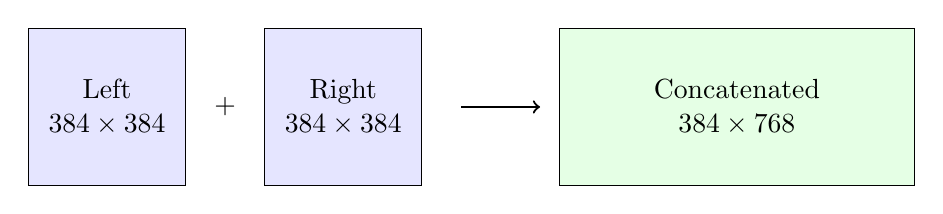
\begin{tikzpicture}[
        img/.style={rectangle, draw, minimum width=2cm, minimum height=2cm, align=center},
        arrow/.style={->, thick}
    ]
        \node[img, fill=blue!10] (left) at (0,0) {Left\\$384 \times 384$};
        \node[img, fill=blue!10] (right) at (3,0) {Right\\$384 \times 384$};
        \node at (1.5,0) {$+$};
        \node[img, fill=green!10, minimum width=4.5cm] (concat) at (8,0) {Concatenated\\$384 \times 768$};

        \draw[arrow] (4.5,0) -- (5.5,0);
    \end{tikzpicture}
    \end{center}

    \vspace{0.5cm}
    \textbf{Processing Steps:}
    \begin{enumerate}
        \item Camera captures at $1280 \times 1024$
        \item Resize to $384 \times 384$ per camera
        \item Concatenate horizontally: $384 \times 768 \times 3$
        \item Optional JPEG compression (training augmentation)
    \end{enumerate}

    \vspace{0.3cm}
    \begin{block}{Camera Order}
        Left image $\rightarrow$ Right image (spatial alignment)
    \end{block}
\end{frame}

%------------------------------------------------------------------------------
\begin{frame}{Chat Template Format}
    \textbf{Qwen2.5-VL Chat Structure:}

    \vspace{0.3cm}
    \begin{lstlisting}[language=Python, basicstyle=\ttfamily\scriptsize]
messages = [{
    "role": "user",
    "content": [
        {"type": "image", "image": concatenated_image},
        {"type": "text", "text": instruction}
    ]
}]

# Apply chat template
text = processor.apply_chat_template(
    messages,
    tokenize=False,
    add_generation_prompt=True
)

# Add action generation markers
text += "<|im_start|>assistant\n<|quad_start|>"
    \end{lstlisting}

    \vspace{0.3cm}
    \textbf{Special Tokens:}
    \begin{itemize}
        \item \code{<|im\_start|>}: Message start marker
        \item \code{<|im\_end|>}: Message end marker
        \item \code{<|quad\_start|>}: Action sequence start
        \item \code{<|quad\_end|>}: Action sequence end
    \end{itemize}
\end{frame}

%------------------------------------------------------------------------------
\begin{frame}{Token Sequence Structure}
    \textbf{Complete Input Sequence:}

    \vspace{0.3cm}
    \begin{center}
    \begin{tikzpicture}[
        tok/.style={rectangle, draw, minimum width=1.2cm, minimum height=0.6cm, align=center, font=\scriptsize},
        arrow/.style={->, thick}
    ]
        \node[tok, fill=gray!30] (sys) at (0,0) {System};
        \node[tok, fill=blue!20] (img) at (1.8,0) {Image\\Tokens};
        \node[tok, fill=green!20] (text) at (3.6,0) {Text\\Tokens};
        \node[tok, fill=yellow!30] (start) at (5.4,0) {quad\\start};
        \node[tok, fill=vqpurple!30] (act) at (7.2,0) {Action\\Tokens};
        \node[tok, fill=yellow!30] (end) at (9,0) {quad\\end};

        \draw[decorate, decoration={brace, amplitude=5pt, raise=2pt}]
            (sys.north west) -- (start.north east) node[midway, above=8pt] {Input Context};

        \draw[decorate, decoration={brace, amplitude=5pt, raise=2pt}]
            (act.north west) -- (end.north east) node[midway, above=8pt] {Generated};
    \end{tikzpicture}
    \end{center}

    \vspace{0.5cm}
    \textbf{Token Counts:}
    \begin{itemize}
        \item Image tokens: $\sim$1000 (depends on resolution)
        \item Text tokens: Variable (instruction length)
        \item Action tokens: Exactly 27
        \item Total context: $< 2048$ tokens
    \end{itemize}
\end{frame}

%------------------------------------------------------------------------------
\begin{frame}{Autoregressive Generation}
    \begin{block}{Process}
        Generate 27 action tokens one at a time
    \end{block}

    \vspace{0.3cm}
    \textbf{Generation Loop:}
    \begin{algorithmic}[1]
        \State $\vect{h} \leftarrow \text{Encode}(\text{image}, \text{instruction})$
        \State $\vect{t} \leftarrow [\;]$ \Comment{token sequence}
        \For{$i = 1$ to $27$}
            \State $p_i \leftarrow \text{LMHead}(\vect{h})$ \Comment{logits over vocabulary}
            \State $t_i \leftarrow \argmax(p_i)$ \Comment{greedy decoding}
            \State $\vect{t}.\text{append}(t_i)$
            \State $\vect{h} \leftarrow \text{Update}(\vect{h}, t_i)$ \Comment{KV cache update}
        \EndFor
        \State \textbf{Return} $\vect{t}$
    \end{algorithmic}

    \vspace{0.3cm}
    \textbf{Inference Configuration:}
    \begin{itemize}
        \item Temperature: $0.0$ (greedy)
        \item Max tokens: 29 (27 + markers)
    \end{itemize}
\end{frame}

%------------------------------------------------------------------------------
\begin{frame}{Token to Action Conversion}
    \textbf{Step 1: Extract Action Tokens}
    \begin{lstlisting}[language=Python, basicstyle=\ttfamily\small]
# Find markers in generated sequence
quad_start = find_token(output, "<|quad_start|>")
quad_end = find_token(output, "<|quad_end|>")
action_tokens = output[quad_start+1 : quad_end]
    \end{lstlisting}

    \vspace{0.3cm}
    \textbf{Step 2: Convert VLA $\rightarrow$ VAE Token IDs}
    \begin{lstlisting}[language=Python, basicstyle=\ttfamily\small]
vocab_size = 152064
vae_tokens = vocab_size - (action_tokens + 1)
vae_tokens = vae_tokens.clamp(0, 1023)
    \end{lstlisting}

    \vspace{0.3cm}
    \textbf{Step 3: Decode via VQVAE}
    \begin{lstlisting}[language=Python, basicstyle=\ttfamily\small]
actions = vae.decode(vae_tokens)  # [B, 24, 20]
    \end{lstlisting}

    \vspace{0.3cm}
    \textbf{Step 4: Unnormalize}
    \begin{lstlisting}[language=Python, basicstyle=\ttfamily\small]
actions = normalizer["action"].unnormalize(actions)
    \end{lstlisting}
\end{frame}

%------------------------------------------------------------------------------
\begin{frame}{Valid Token Rate}
    \begin{block}{Quality Metric}
        Percentage of generated tokens within valid codebook range
    \end{block}

    \vspace{0.3cm}
    \textbf{Definition:}
    \[
        \text{valid\_rate} = \frac{|\{t : 0 \leq t < 1024\}|}{27}
    \]

    \vspace{0.3cm}
    \textbf{Invalid Token Causes:}
    \begin{itemize}
        \item Model generates text tokens instead of action tokens
        \item Token ID outside codebook range after conversion
        \item Premature \code{<|quad\_end|>} generation
    \end{itemize}

    \vspace{0.3cm}
    \begin{alertblock}{Handling Invalid Tokens}
        \begin{itemize}
            \item Clamp to valid range: $[0, 1023]$
            \item Monitor valid\_rate during training/inference
            \item Low valid\_rate indicates training issues
        \end{itemize}
    \end{alertblock}
\end{frame}

%------------------------------------------------------------------------------
\begin{frame}{Training: Loss Function}
    \textbf{Cross-Entropy Loss on Action Tokens:}

    \vspace{0.3cm}
    \[
        \mathcal{L}_{\text{CE}} = -\sum_{i=1}^{27} \log P(t_i | t_{<i}, \text{image}, \text{instruction})
    \]

    \vspace{0.5cm}
    \textbf{Label Preparation:}
    \begin{enumerate}
        \item Encode ground-truth actions: $\vect{a} \rightarrow \vect{t}_{\text{gt}}$ via VQVAE
        \item Convert to VLA token IDs: $t_{\text{vla}} = V - t_{\text{vae}} - 1$
        \item Mask non-action positions: $-100$ (ignored in loss)
    \end{enumerate}

    \vspace{0.3cm}
    \textbf{Training Configuration:}
    \begin{itemize}
        \item Only action token positions contribute to loss
        \item Image/text tokens are input context only
        \item Teacher forcing: ground-truth tokens as input
    \end{itemize}
\end{frame}

%------------------------------------------------------------------------------
\begin{frame}{Training: LoRA Configuration}
    \begin{block}{Parameter-Efficient Fine-Tuning}
        LoRA adapters on attention layers
    \end{block}

    \vspace{0.3cm}
    \textbf{Target Modules:}
    \begin{lstlisting}[language=Python, basicstyle=\ttfamily\small]
LoraConfig(
    r=8,                    # LoRA rank
    lora_alpha=8,           # Scaling factor
    lora_dropout=0.1,       # Dropout rate
    target_modules=[
        "q_proj", "k_proj", "v_proj", "o_proj",
        "gate_proj", "up_proj", "down_proj"
    ],
    use_dora=False,
    init_lora_weights="gaussian"
)
    \end{lstlisting}

    \vspace{0.3cm}
    \textbf{Trainable Parameters:}
    \begin{itemize}
        \item LoRA: $\sim$20M parameters (0.3\% of 7B)
        \item Full fine-tune: 7B parameters
    \end{itemize}
\end{frame}

%------------------------------------------------------------------------------
\begin{frame}{Training: QLoRA Configuration}
    \begin{block}{Quantized LoRA}
        4-bit quantization + LoRA for memory efficiency
    \end{block}

    \vspace{0.3cm}
    \textbf{Quantization Config:}
    \begin{lstlisting}[language=Python, basicstyle=\ttfamily\small]
BitsAndBytesConfig(
    load_in_4bit=True,
    bnb_4bit_use_double_quant=True,
    bnb_4bit_quant_type="nf4",
    bnb_4bit_compute_dtype=torch.bfloat16
)
    \end{lstlisting}

    \vspace{0.3cm}
    \textbf{LoRA with DoRA:}
    \begin{lstlisting}[language=Python, basicstyle=\ttfamily\small]
LoraConfig(
    ...,
    use_dora=True  # Weight decomposition
)
    \end{lstlisting}

    \vspace{0.3cm}
    \textbf{Memory Comparison:}
    \begin{itemize}
        \item Full: $\sim$80 GB VRAM
        \item LoRA: $\sim$32 GB VRAM
        \item QLoRA: $\sim$20 GB VRAM
    \end{itemize}
\end{frame}

%------------------------------------------------------------------------------
\begin{frame}{Evaluation Metrics}
    \textbf{Computed during training/validation:}

    \vspace{0.5cm}
    \begin{table}
        \centering
        \renewcommand{\arraystretch}{1.3}
        \begin{tabular}{ll}
            \toprule
            \textbf{Metric} & \textbf{Formula} \\
            \midrule
            Valid Rate & $\frac{\text{\# valid tokens}}{27}$ \\[0.3cm]
            MSE (Total) & $\|\hat{\vect{a}} - \vect{a}\|^2$ \\[0.3cm]
            MSE (Position) & $\|\hat{\vect{p}} - \vect{p}\|^2$ \\[0.3cm]
            Geodesic (Rotation) & $\arccos\left(\frac{\text{tr}(\mat{R}^T \hat{\mat{R}}) - 1}{2}\right)$ \\[0.3cm]
            MSE (Gripper) & $\|\hat{g} - g\|^2$ \\
            \bottomrule
        \end{tabular}
    \end{table}

    \vspace{0.3cm}
    \begin{block}{Note}
        Metrics computed on unnormalized actions for interpretability
    \end{block}
\end{frame}

%------------------------------------------------------------------------------
\begin{frame}{vLLM Acceleration}
    \begin{block}{Purpose}
        Faster inference using optimized LLM serving
    \end{block}

    \vspace{0.3cm}
    \textbf{vLLM Configuration:}
    \begin{lstlisting}[language=Python, basicstyle=\ttfamily\small]
from vllm import LLM, SamplingParams

llm = LLM(
    model=model_path,
    dtype=torch.bfloat16,
    tensor_parallel_size=1,
    enable_chunked_prefill=True,
    gpu_memory_utilization=0.90,
    max_model_len=2048,
    limit_mm_per_prompt={"image": 1}
)

sampling_params = SamplingParams(
    max_tokens=29,
    temperature=0.0
)
    \end{lstlisting}
\end{frame}

%------------------------------------------------------------------------------
\begin{frame}{vLLM Inference}
    \textbf{Inference with vLLM:}

    \vspace{0.3cm}
    \begin{lstlisting}[language=Python, basicstyle=\ttfamily\small]
# Prepare input
prompt = build_chat_template(image, instruction)

# Generate
outputs = llm.generate(
    prompts=[prompt],
    sampling_params=sampling_params,
    use_tqdm=False
)

# Extract tokens (no detokenization)
token_ids = outputs[0].outputs[0].token_ids
    \end{lstlisting}

    \vspace{0.5cm}
    \textbf{Performance:}
    \begin{itemize}
        \item Standard HuggingFace: $\sim$400ms per inference
        \item vLLM: $\sim$237ms per inference
        \item Speedup: $\sim$1.7$\times$
    \end{itemize}
\end{frame}

%------------------------------------------------------------------------------
\begin{frame}{KV Cache Optimization}
    \begin{block}{Key Insight}
        Image/text encoding is constant across action tokens
    \end{block}

    \vspace{0.3cm}
    \textbf{Standard Generation:}
    \begin{itemize}
        \item Each token: Full forward pass
        \item Total: $27 \times$ full computation
    \end{itemize}

    \vspace{0.3cm}
    \textbf{With KV Cache:}
    \begin{itemize}
        \item First token: Full forward (encode image + text)
        \item Subsequent tokens: Only decode new token
        \item KV cache stores attention states
    \end{itemize}

    \vspace{0.3cm}
    \textbf{Implementation:}
    \begin{lstlisting}[language=Python, basicstyle=\ttfamily\small]
# Initial encoding
outputs = model(**inputs, use_cache=True)
past_key_values = outputs.past_key_values

# Subsequent generation
outputs = model(input_ids=new_token,
                past_key_values=past_key_values)
    \end{lstlisting}
\end{frame}

%------------------------------------------------------------------------------
\begin{frame}{RDT2-VQ Strengths \& Weaknesses}
    \begin{columns}[T]
        \begin{column}{0.5\textwidth}
            \textbf{Strengths:}
            \begin{itemize}
                \item Full VLM language understanding
                \item Superior instruction following
                \item Unified text-action interface
                \item Stable discrete training
                \item Leverages pretrained VLM
            \end{itemize}
        \end{column}
        \begin{column}{0.5\textwidth}
            \textbf{Weaknesses:}
            \begin{itemize}
                \item 27 forward passes (slow)
                \item Discretization error
                \item High memory usage
                \item Sequential generation
                \item Cannot parallelize tokens
            \end{itemize}
        \end{column}
    \end{columns}

    \vspace{0.5cm}
    \begin{alertblock}{Latency Analysis}
        27 forward passes $\times$ $\sim$15ms = $\sim$400ms per action chunk \\
        Action chunk = 0.8s $\Rightarrow$ \textbf{50\% of real-time}
    \end{alertblock}
\end{frame}

%------------------------------------------------------------------------------
\begin{frame}{HuggingFace Model}
    \textbf{Model Location:}

    \vspace{0.3cm}
    \code{robotics-diffusion-transformer/RDT2-VQ}

    \vspace{0.5cm}
    \textbf{Loading:}
    \begin{lstlisting}[language=Python, basicstyle=\ttfamily\small]
from transformers import (
    Qwen2_5_VLForConditionalGeneration,
    AutoProcessor
)

model = Qwen2_5_VLForConditionalGeneration \
    .from_pretrained(
        "robotics-diffusion-transformer/RDT2-VQ",
        torch_dtype=torch.bfloat16,
        attn_implementation="flash_attention_2"
    )

processor = AutoProcessor.from_pretrained(
    "Qwen/Qwen2.5-VL-7B-Instruct"
)
    \end{lstlisting}
\end{frame}

%------------------------------------------------------------------------------
\begin{frame}{Complete Inference Pipeline}
    \begin{center}
    \begin{tikzpicture}[
        box/.style={rectangle, draw, rounded corners, minimum width=2cm, minimum height=0.6cm, align=center, font=\scriptsize},
        arrow/.style={->, thick},
        scale=0.75, transform shape
    ]
        % Row 1: Input
        \node[box, fill=blue!20] (img) at (0,4) {Images\\$2 \times 384^2$};
        \node[box, fill=green!20] (inst) at (3,4) {Instruction};
        \node[box, fill=gray!30] (proc) at (6,4) {Processor};

        % Row 2: Model
        \node[box, fill=qwenblue!30, minimum width=6cm] (qwen) at (4.5,2) {Qwen2.5-VL-7B (27 forward passes)};

        % Row 3: Tokens
        \node[box, fill=vqpurple!30] (vla_tok) at (0,0) {VLA Tokens\\$[27]$};
        \node[box, fill=gray!30] (convert) at (3,0) {Convert\\$V - t - 1$};
        \node[box, fill=vqpurple!30] (vae_tok) at (6,0) {VAE Tokens\\$[27]$};

        % Row 4: Decode
        \node[box, fill=yellow!30] (vae) at (9,0) {VQVAE\\Decode};
        \node[box, fill=actionorange!30] (norm_act) at (12,0) {Normalized\\$[24,20]$};

        % Row 5: Output
        \node[box, fill=gray!30] (unnorm) at (12,-2) {Unnormalize};
        \node[box, fill=rdtgreen!30] (action) at (9,-2) {Action\\$[24,20]$};

        % Arrows
        \draw[arrow] (img) -- (proc);
        \draw[arrow] (inst) -- (proc);
        \draw[arrow] (proc) -- (qwen);
        \draw[arrow] (qwen) -- (vla_tok);
        \draw[arrow] (vla_tok) -- (convert);
        \draw[arrow] (convert) -- (vae_tok);
        \draw[arrow] (vae_tok) -- (vae);
        \draw[arrow] (vae) -- (norm_act);
        \draw[arrow] (norm_act) -- (unnorm);
        \draw[arrow] (unnorm) -- (action);
    \end{tikzpicture}
    \end{center}

    \vspace{0.3cm}
    \textbf{Total Latency:} $\sim$400ms (without vLLM) / $\sim$237ms (with vLLM)
\end{frame}

%------------------------------------------------------------------------------
\begin{frame}{RDT2-VQ Summary}
    \begin{table}
        \centering
        \renewcommand{\arraystretch}{1.3}
        \begin{tabular}{ll}
            \toprule
            \textbf{Attribute} & \textbf{Value} \\
            \midrule
            Backbone & Qwen2.5-VL-7B-Instruct \\
            Output type & Discrete tokens \\
            Tokens per chunk & 27 \\
            Forward passes & 27 \\
            Action chunk & 24 frames (0.8s) \\
            Inference time & $\sim$400ms (standard) \\
            Training modes & Full / LoRA / QLoRA \\
            \bottomrule
        \end{tabular}
    \end{table}

    \vspace{0.5cm}
    \begin{block}{Use Case}
        Best for tasks requiring strong language understanding and instruction following, where latency is acceptable
    \end{block}
\end{frame}

